\documentclass[11pt,letterpaper]{article}
\usepackage[T1]{fontenc}
\usepackage[utf8]{inputenc}
\usepackage{newpxtext}
\usepackage[margin=0.92in,headheight=15pt]{geometry}
\usepackage{microtype}
\usepackage{mathtools,amsthm,amssymb}
\usepackage{newpxmath}
\usepackage{booktabs,array,graphicx}
\usepackage{xcolor}
\usepackage{enumitem}
\usepackage{listings}
\usepackage{fancyhdr}
\usepackage{titlesec}
\usepackage{hyperref}
\definecolor{accent}{HTML}{42564A}
\definecolor{codebg}{HTML}{F5F5F1}
\hypersetup{colorlinks=true,linkcolor=accent,citecolor=accent,urlcolor=accent,
  pdftitle={A Mixed-Base Counterexample to Stanley's Rationality Question},
  pdfauthor={Research report prepared for Vladimir Reshetnikov},
  pdfsubject={Exact coefficient counts, irrational thresholds, and a natural boundary}}
\titleformat{\section}{\large\bfseries\color{accent}}{\thesection}{0.65em}{}
\titleformat{\subsection}{\normalsize\bfseries}{\thesubsection}{0.65em}{}
\pagestyle{fancy}
\fancyhf{}
\fancyhead[L]{\small A mixed-base counterexample}
\fancyhead[R]{\small Exact counts and natural boundaries}
\fancyfoot[C]{\thepage}
\renewcommand{\headrulewidth}{0.3pt}
\setlength{\parskip}{4pt}
\setlength{\parindent}{1.2em}
\setlength{\emergencystretch}{2em}
\raggedbottom
\clubpenalty=5000
\widowpenalty=5000
\setcounter{tocdepth}{1}
\numberwithin{equation}{section}
\newtheorem{theorem}{Theorem}[section]
\newtheorem{lemma}[theorem]{Lemma}
\newtheorem{proposition}[theorem]{Proposition}
\newtheorem{corollary}[theorem]{Corollary}
\theoremstyle{definition}
\newtheorem{definition}[theorem]{Definition}
\newtheorem{example}[theorem]{Example}
\theoremstyle{remark}
\newtheorem{remark}[theorem]{Remark}
\newcommand{\N}{\mathbb{N}}
\newcommand{\Z}{\mathbb{Z}}
\newcommand{\Q}{\mathbb{Q}}
\newcommand{\C}{\mathbb{C}}
\newcommand{\F}{\mathbb{F}}
\newcommand{\ind}[1]{\boldsymbol{1}_{\{#1\}}}
\newcommand{\fracpart}[1]{\left\{#1\right\}}
\newcommand{\floor}[1]{\left\lfloor#1\right\rfloor}
\newcommand{\ceil}[1]{\left\lceil#1\right\rceil}
\newcommand{\coeff}[2]{[x^{#1}]#2}
\DeclareMathOperator{\lcm}{lcm}
\lstset{language=Python,basicstyle=\small\ttfamily,columns=fullflexible,
  keepspaces=true,showstringspaces=false,breaklines=true,
  backgroundcolor=\color{codebg},frame=single,rulecolor=\color{black!15},
  xleftmargin=0.4em,xrightmargin=0.4em,aboveskip=10pt,belowskip=8pt}
\title{\vspace{-1.4em}\textbf{A Mixed-Base Counterexample to\\
Stanley's Rationality Question}\\[0.35em]
\large Exact coefficient counts, irrational thresholds,\\and a natural boundary}
\author{\normalsize Research report prepared for Vladimir Reshetnikov}
\date{\normalsize September 19, 2026}

\begin{document}
\maketitle
\vspace{-1.2em}
\begin{abstract}
Richard Stanley asked whether a positive integer sequence tending to infinity
and having a rational generating function necessarily produces rational
generating functions for the numbers of coefficients equal to a fixed integer
in its associated finite products. We give a counterexample using the
interleaved sequences $2^j$ and $3^j$. For
$P_N(x)=\prod_{i=1}^N(1+x^{G_i})$, with $G_{2j+1}=2^j$ and
$G_{2j+2}=3^j$, the number $a_n$ of coefficients equal to $1$ in $P_{2n}$ is
\[
 a_n=2^{\,n-\lfloor(n+1)\log_3 2\rfloor}+\ind{n=1}.
\]
The proof turns polynomial coefficients into interval-covering
multiplicities and then counts gaps created by ternary carries.
A finite-field argument proves nonrationality without any transcendence
assumption about the exponential growth constant. A separate analytic argument
proves a natural boundary, hence non-D-finiteness and the absence of
polynomial-coefficient linear recurrences. Finally, for a two-base family
with digits $0,\ldots,a-1$, we prove that rationality holds exactly when
the bases are multiplicatively dependent. Exact-integer verification code,
sequence data, and reproducible figures accompany the proofs.
\end{abstract}
\vspace{-0.6em}
\begingroup
\small
\setlength{\parskip}{0pt}
\tableofcontents
\endgroup
\clearpage

\section{The problem and the result}\label{sec:problem}

In a MathOverflow question dated September 23, 2022, Richard Stanley considers
a sequence of positive integers $(G_N)_{N\ge1}$ satisfying
\begin{equation}\label{eq:hypotheses}
 G_N\longrightarrow\infty,
 \qquad \sum_{N\ge1}G_Nt^N\in\Q(t).
\end{equation}
For a fixed integer $r\ge1$, put
\begin{equation}\label{eq:stanleyproduct}
 P_N(x)=\prod_{i=1}^N\bigl(1+x^{G_i}+\cdots+x^{rG_i}\bigr),
 \qquad P_0(x)=1.
\end{equation}
For fixed $k\ge1$, let $\nu_k(N)$ be the number of exponents $s\ge0$ for
which $[x^s]P_N(x)=k$. The question asks whether
$\sum_{N\ge0}\nu_k(N)t^N$ is rational and, if not universally, which
sequences $G_N$ have this property \cite{StanleyMO}.

The present report gives a negative answer to the universal assertion,
already for $r=k=1$. The source question requires divergence to infinity,
\emph{not monotonicity}. That distinction matters: the counterexample below
is not monotone.

\subsection{An explicit counterexample}
For every $j\ge0$, define
\begin{equation}\label{eq:exponents}
 G_{2j+1}=2^j,\qquad G_{2j+2}=3^j.
\end{equation}
Thus the beginning of the exponent sequence is
\[
 1,1,2,3,4,9,8,27,16,81,32,243,\ldots.
\]
Its generating function is visibly rational:
\begin{equation}\label{eq:inputgf}
 \sum_{N\ge1}G_Nt^N
 =\frac{t}{1-2t^2}+\frac{t^2}{1-3t^2}
 =\frac{t+t^2-3t^3-2t^4}{1-5t^2+6t^4}.
\end{equation}
Equivalently,
\begin{equation}\label{eq:inputrec}
 G_{N+4}=5G_{N+2}-6G_N\qquad(N\ge1).
\end{equation}
Both parity subsequences tend to infinity, so \eqref{eq:hypotheses} holds.
Write
\begin{equation}\label{eq:ABF}
 \nu(N)=\nu_1(N),\quad a_n=\nu(2n),\quad b_n=\nu(2n+1),
 \quad A(z)=\sum_{n\ge0}a_nz^n,\quad F(t)=\sum_{N\ge0}\nu(N)t^N.
\end{equation}
The variable $x$ always records polynomial exponents; $z$ and $t$ record
product lengths. In particular, $A$ is a section of $F$, not a specialization
of the product variable $x$.

\begin{theorem}[Counterexample and analytic strengthening]\label{thm:main}
Set $\alpha=\log_3 2$ and $R=2^{\alpha-1}$. For the exponents
\eqref{eq:exponents},
\begin{equation}\label{eq:mainformula}
 a_n=2^{\,n-\lfloor(n+1)\alpha\rfloor}+\ind{n=1}\qquad(n\ge0).
\end{equation}
Neither $A(z)$ nor $F(t)$ is rational. In fact, $|z|=R$ is a natural boundary
for $A$, and $|t|=\sqrt R$ is a natural boundary for $F$. Consequently both
functions are non-D-finite and transcendental over their rational function
fields, and neither coefficient sequence is P-recursive.
\end{theorem}

The elementary counterexample is complete by Section~\ref{sec:nonrational}.
Sections~\ref{sec:floor}--\ref{sec:boundary} establish the exact floor formula
and the stronger analytic conclusions. Section~\ref{sec:general} proves a
necessary-and-sufficient condition for rationality in a broader two-base
family.

\subsection{Source status and scope of the claim}
The source page displayed no posted answer when inspected on September 19,
2026. Targeted searches for the question title, its identifier, and mixed-base
counterexamples did not reveal an existing resolution. This is a limited
literature audit, not a proof of priority. The mathematical assertions here
are supported by the proofs below; the report has not been independently
refereed or formally verified in a proof assistant.

Stanley's related work on rational generating functions for moments of
polynomial coefficients supplies useful context \cite{StanleyRational}.
Those moment questions and the fixed-multiplicity question
\eqref{eq:stanleyproduct} are different. This report does not claim to
contradict a theorem or settle the other conjectures in that paper.

\section{From polynomial coefficients to interval coverage}\label{sec:intervals}

The basic mechanism is that one half of the product creates a solid interval
of monomials, while the other half creates a sparse set of translates.
Counting coefficients equal to one then becomes a geometric counting problem
on the integer line.

\subsection{A general unique-coverage identity}
Let $s_0<s_1<\cdots<s_{M-1}$ be integer starting points, $M\ge2$, and let
$L\ge1$ be an integer. Consider the half-open intervals
\[
 I_i=[s_i,s_i+L),\qquad 0\le i<M.
\]
Only their integer points are counted. Write
$d_i=s_{i+1}-s_i$ for $0\le i<M-1$.

\begin{lemma}[Unique coverage]\label{lem:coverage}
The number of integers belonging to exactly one of the intervals $I_i$ is
\begin{equation}\label{eq:coverage}
 \min(d_0,L)+\min(d_{M-2},L)
 +\sum_{i=1}^{M-2}
 \max\!\bigl(0,\min(d_{i-1},L)+\min(d_i,L)-L\bigr).
\end{equation}
The sum is empty when $M=2$.
\end{lemma}
\begin{proof}
An integer in $I_0$ belongs to no other interval exactly when it is smaller
than $s_1$. There are $\min(d_0,L)$ such integers. The last interval similarly
contributes $\min(d_{M-2},L)$.

Now fix an internal interval $I_i$. Because all intervals have the same
length, the immediate predecessor has the rightmost endpoint among all
previous intervals, and the immediate successor has the leftmost starting
point among all later ones. An integer in $I_i$ therefore belongs to no other
interval exactly when it lies in
\[
 [\max(s_i,s_{i-1}+L),\ \min(s_i+L,s_{i+1})).
\]
The endpoints are integers. Its number of integer points is its length when
positive, and zero otherwise. Subtracting $s_i$ from both endpoints gives
\[
 \max\bigl(0,\min(L,d_i)-\max(0,L-d_{i-1})\bigr),
\]
which is the corresponding summand in \eqref{eq:coverage}. Each uniquely
covered point belongs to exactly one interval, so these contributions are
disjoint and exhaustive.
\end{proof}

\begin{corollary}[Isolated large gaps]\label{cor:isolated}
Suppose $L\ge2$, the first and last gaps are $1$, and no two gaps greater
than $1$ are adjacent. If $H$ gaps have size at least $L$, the number of
uniquely covered integers is
\begin{equation}\label{eq:isolated}
 2+2H.
\end{equation}
\end{corollary}
\begin{proof}
The two boundary terms in \eqref{eq:coverage} are $1$. For an internal
interval at least one neighboring gap is $1$. If the other gap is $g$, the
contribution is
\[
 \max(0,1+\min(g,L)-L).
\]
As $g$ and $L$ are integers, this is $1$ exactly when $g\ge L$, and is zero
otherwise. Each gap of size at least $L$ is nonunit, is not a boundary gap,
and borders two internal intervals. It therefore contributes twice.
\end{proof}

\subsection{The rectangular binary--ternary product}
For $m,n\ge0$, define
\begin{equation}\label{eq:rectangle}
 Q_{m,n}(x)=
 \prod_{j=0}^{m-1}(1+x^{2^j})
 \prod_{j=0}^{n-1}(1+x^{3^j}).
\end{equation}
The first product enumerates all binary expansions of length $m$, uniquely,
so
\begin{equation}\label{eq:densefactor}
 \prod_{j=0}^{m-1}(1+x^{2^j})=1+x+\cdots+x^{2^m-1}.
\end{equation}
The second product has coefficient $1$ precisely at the points of
\begin{equation}\label{eq:ternarysupport}
 S_n=\left\{\sum_{j=0}^{n-1}\epsilon_j3^j:
             \epsilon_j\in\{0,1\}\right\},
 \qquad |S_n|=2^n.
\end{equation}
Ternary expansions are unique, so there is no multiplicity within $S_n$.
Consequently
\begin{equation}\label{eq:coverageinterpretation}
 [x^s]Q_{m,n}(x)=\#\{u\in S_n:u\le s<u+2^m\}.
\end{equation}
This identity reduces the coefficient problem exactly, not approximately,
to Lemma~\ref{lem:coverage} with interval length $L=2^m$.

\section{Ternary carries and exact counts}\label{sec:exact}

\subsection{The complete gap distribution}
The elements of $S_n$ are sorted by interpreting the binary digit strings
$\epsilon_{n-1}\cdots\epsilon_0$ as ternary strings. This preserves their
order: changing the highest differing digit outweighs all lower digits.

\begin{lemma}[Ternary support gaps]\label{lem:ternarygaps}
For $n\ge1$, the gaps between consecutive elements of $S_n$ have sizes
\begin{equation}\label{eq:ternarygap}
 g_t=\frac{3^t+1}{2},\qquad 0\le t<n.
\end{equation}
The gap $g_t$ occurs $2^{n-1-t}$ times. The first and last gaps are $1$,
and every pair of adjacent gaps contains a gap of size $1$.
\end{lemma}
\begin{proof}
To move to the next binary digit string, turn a string of $t$ trailing ones
into zeroes and turn the next zero into a one. The corresponding change in
the ternary value is
\[
 3^t-\sum_{j=0}^{t-1}3^j
 =3^t-\frac{3^t-1}{2}=\frac{3^t+1}{2}.
\]
For a carry of length $t$, the $t$ trailing digits and the next digit are
fixed, while the $n-1-t$ higher digits are arbitrary. This gives the stated
multiplicity. A nontrivial carry resets the last digit to zero, so the next
step changes only that digit and has gap $1$. The step immediately before
a nontrivial carry is also a unit step. The first and last steps both change
only the last digit. These observations establish the adjacency and boundary
claims.
\end{proof}

The multiplicities sum to $2^n-1$, as required. Although the largest gap
grows exponentially, gaps larger than one remain separated by unit gaps.
That separation is what makes the number of coefficients equal to one simple.

\subsection{An exact integer threshold}
Define
\begin{equation}\label{eq:threshold}
 T(m)=\min\{t\ge0:3^t\ge 2^{m+1}-1\}.
\end{equation}
For $m\ge1$, this is at least $1$. Let $U(m,n)$ denote the number of
coefficients equal to one in $Q_{m,n}$.

\begin{theorem}[Rectangular count]\label{thm:rectangle}
For $m,n\ge1$,
\begin{equation}\label{eq:rectcount}
 U(m,n)=2^{\,1+\max(0,n-T(m))}.
\end{equation}
The boundary cases are
\begin{equation}\label{eq:rectboundary}
 U(m,0)=2^m,\qquad U(0,n)=2^n.
\end{equation}
In particular $U(0,0)=1$.
\end{theorem}
\begin{proof}
A gap $g_t$ is at least $2^m$ exactly when $t\ge T(m)$. If $T(m)<n$,
Lemma~\ref{lem:ternarygaps} gives
\[
 H=\sum_{t=T(m)}^{n-1}2^{n-1-t}=2^{n-T(m)}-1.
\]
If $T(m)\ge n$, then $H=0$. Apply Corollary~\ref{cor:isolated} and simplify
$2+2H$. When one of the products is empty, the other has all its nonzero
coefficients equal to one, proving \eqref{eq:rectboundary}.
\end{proof}

Since $P_{2n}=Q_{n,n}$ and $P_{2n+1}=Q_{n+1,n}$, this already determines
the entire sequence $\nu(N)$ by integer arithmetic.
For $n\ge1$, the inequality
\begin{equation}\label{eq:diagonalthreshold}
 3^n+1\ge2^{n+1}
\end{equation}
holds by induction, so $T(n)\le n$. Thus
\begin{equation}\label{eq:diagonalcount}
 a_0=1,\qquad a_n=2^{\,n-T(n)+1}\quad(n\ge1).
\end{equation}
The first values are given in Table~\ref{tab:terms}. In the table $T(0)=0$;
formula \eqref{eq:diagonalcount} has its stated separate case at $n=0$.

\begin{table}[htbp]
\centering
\caption{Exact counts on the even subsequence.}\label{tab:terms}
\begin{tabular}{rrr@{\qquad}rrr@{\qquad}rrr}
\toprule
$n$&$T(n)$&$a_n$&$n$&$T(n)$&$a_n$&$n$&$T(n)$&$a_n$\\
\midrule
0&0&1&  7&6&4& 14&10&32\\
1&1&2&  8&6&8& 15&11&32\\
2&2&2&  9&7&8& 16&11&64\\
3&3&2& 10&7&16& 17&12&64\\
4&4&2& 11&8&16& 18&12&128\\
5&4&4& 12&9&16& 19&13&128\\
6&5&4& 13&9&32& 20&14&128\\
\bottomrule
\end{tabular}
\end{table}

\subsection{A fully visible example}
Take $m=n=5$. The interval length is $32$, while the gap sizes are
$1,2,5,14,41$. Only the gap $41$ reaches the threshold; it occurs once.
Therefore $U(5,5)=2+2=4$.

Concretely, the support $S_5$ splits into a block ending at
$1+3+9+27=40$ and a block beginning at $81$. The first block's final
interval ends just after $71$, while the second block starts at $81$.
The four uniquely covered integers are
\begin{equation}\label{eq:examplelocations}
 0,\quad71,\quad81,\quad152.
\end{equation}
The outer two come from the global boundaries, and the middle two flank
the unique large gap. Direct multiplication of $P_{10}$ gives precisely
these coefficient-one positions; Figure~\ref{fig:profile} displays all
coefficients, including the zero coefficients between the two blocks.

\begin{figure}[htbp]
\centering
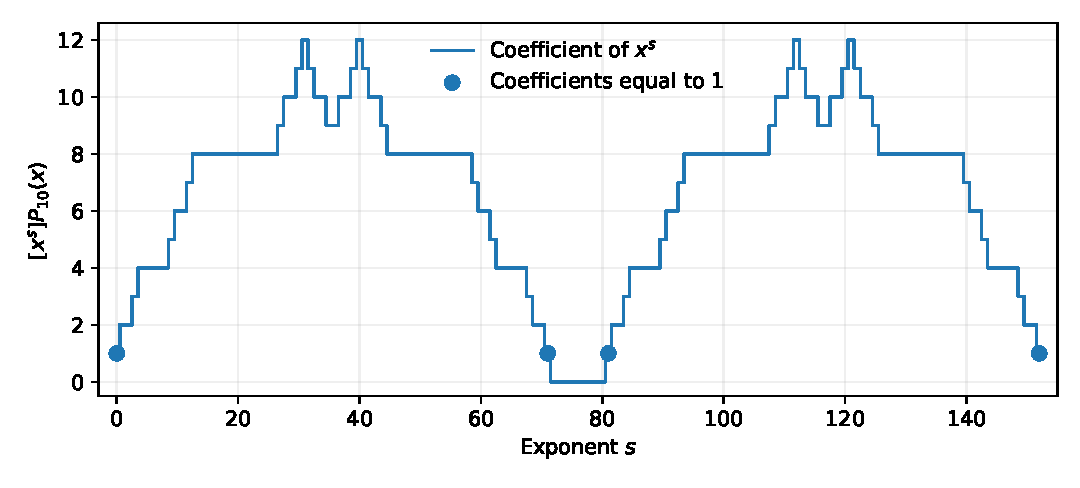
\includegraphics[width=0.97\linewidth]{figures/coefficient_profile.pdf}
\caption{The coefficients of $P_{10}=Q_{5,5}$. The four marked values occur
at the positions in \eqref{eq:examplelocations}. The maximum coefficient
is $12$; the sum of all coefficients is $2^{10}=1024$.}
\label{fig:profile}
\end{figure}

\section{An elementary obstruction to rationality}\label{sec:nonrational}

The exact count is a power of two. Its exponent grows at an irrational
average speed but changes only by zero or one at each step. Rational
generating functions cannot exhibit this particular combination.

\subsection{Rational recurrences modulo a prime}
A sequence is called \emph{C-finite} when, from some index onward, it
satisfies a linear recurrence with constant coefficients. An ordinary
generating function over $\Q$ is rational if and only if its coefficients
are C-finite over $\Q$: multiplying the series by its denominator gives
the recurrence, and summing an eventual recurrence gives a polynomial
numerator divided by a polynomial denominator.

There is no change in this conclusion if rationality is initially allowed
over $\C$ for a series with rational coefficients. For a fixed denominator
degree and a fixed numerator bound, the coefficient identities are linear
equations with rational entries in finitely many unknown denominator
coefficients, with the constant denominator coefficient normalized to one.
A finite subsystem spans all the augmented rows. If a complex solution
exists, rational Gaussian elimination gives a rational solution to that
subsystem and hence to all the identities. Thus the rational function can
be taken over $\Q$.

\begin{lemma}[Finite ratios and irrational exponent slope]\label{lem:finitefield}
Let $b\ge2$ and $C\ge1$ be integers. Suppose an integer sequence $(u_n)$
has, for all sufficiently large $n$, the form
\[
 u_n=C b^{e_n},\qquad e_n\in\Z_{\ge0},\qquad e_{n+1}-e_n\in\{0,1\}.
\]
If $\lim_{n\to\infty}e_n/n$ exists and is irrational, then
$\sum_{n\ge0}u_nz^n$ is not rational.
\end{lemma}
\begin{proof}
Suppose the generating function were rational. Then for some $d\ge1$
and rational constants $c_0,\ldots,c_{d-1}$,
\begin{equation}\label{eq:rationalrec}
 u_{n+d}=c_{d-1}u_{n+d-1}+\cdots+c_0u_n
\end{equation}
for every sufficiently large $n$. Choose a prime $p$ dividing neither
$Cb(b-1)$ nor any denominator of the $c_j$. Only finitely many primes
are excluded.

Reduce \eqref{eq:rationalrec} modulo $p$. The state vector
$(u_n,\ldots,u_{n+d-1})\bmod p$ belongs to the finite set $\F_p^d$ and
has a deterministic successor. Its forward orbit, and hence $u_n\bmod p$,
is eventually periodic. No invertibility of the transition is needed.

For large $n$, all $u_n\bmod p$ are nonzero. The quotient
$u_{n+1}/u_n\bmod p$ is therefore eventually periodic as well. Its actual
integer value is either $1$ or $b$, and these have distinct residues modulo
$p$. The periodic residue quotient thus uniquely determines the actual
quotient. Consequently $e_{n+1}-e_n$ is eventually periodic.

If its eventual period has length $L$ and contains $J$ ones, summing the
increments yields $e_n=(J/L)n+O(1)$. The limit $e_n/n$ must be the rational
number $J/L$, contrary to the hypothesis.
\end{proof}

\subsection{Applying the obstruction}
By its definition, $T(n)$ is nondecreasing. For $n\ge1$, if
$3^{T(n)}\ge2^{n+1}-1$, then
\[
 3^{T(n)+1}\ge3(2^{n+1}-1)\ge2^{n+2}-1.
\]
Therefore
\begin{equation}\label{eq:thresholdstep}
 T(n+1)-T(n)\in\{0,1\}\qquad(n\ge1).
\end{equation}
Moreover, the two adjacent powers bracketing the threshold give
\begin{equation}\label{eq:thresholdslope}
 T(n)=n\log_3 2+O(1).
\end{equation}
For $n\ge1$ put $e_n=n-T(n)+1$. Equations
\eqref{eq:diagonalcount}, \eqref{eq:thresholdstep}, and
\eqref{eq:thresholdslope} show that
\[
 a_n=2^{e_n},\qquad e_{n+1}-e_n\in\{0,1\},\qquad
 \frac{e_n}{n}\longrightarrow1-\log_3 2.
\]
The last limit is irrational. Indeed, a rational equality
$\log_3 2=p/q$ with positive integers $p,q$ would imply
$2^q=3^p$, contradicting unique prime factorization. Lemma~\ref{lem:finitefield}
proves that $A$ is not rational.

Finally, the even section of a rational series is rational. One way to see
this is to represent an eventual recurrence by a finite companion matrix:
sampling at even indices replaces the matrix by its square and again gives
a constant-coefficient recurrence, by the characteristic polynomial.
Equivalently,
\[
 \frac{F(t)+F(-t)}2=A(t^2),
\]
and an even rational function of $t$ is a rational function of $t^2$.
Thus rationality of $F$ would imply rationality of $A$, a contradiction.
This proves the negative answer to the universal rationality question.

\begin{remark}[What the argument does not assume]
The irrationality of an exponential growth constant by itself would not
rule out rationality: coefficients of a rational function can have
irrational algebraic exponential growth. The proof instead uses an
irrational \emph{frequency of discrete exponent increments} and finite-state
arithmetic modulo a prime. It makes no algebraicity or transcendence claim
about $2^{1-\log_3 2}$.
\end{remark}

\section{The floor formula and the odd indices}\label{sec:floor}

\subsection{Removing the near-integer ambiguity}
The threshold \eqref{eq:threshold} involves $2^{n+1}-1$, not $2^{n+1}$.
The difference is important for the initial terms and must not be silently
dropped.

\begin{proposition}[Exact floor expression]\label{prop:floor}
For $n\ge2$,
\begin{equation}\label{eq:Tfloor}
 T(n)=\ceil{(n+1)\alpha}=\floor{(n+1)\alpha}+1,
 \qquad \alpha=\log_3 2.
\end{equation}
Consequently \eqref{eq:mainformula} holds for every $n\ge0$.
\end{proposition}
\begin{proof}
Let $M=\ceil{(n+1)\alpha}$ be the least integer such that
$3^M\ge2^{n+1}$. The number $(n+1)\alpha$ is irrational, so the inequality
is strict and the ceiling is one more than the floor.
Since the smaller threshold in \eqref{eq:threshold} is $2^{n+1}-1$,
we have $T(n)\le M$. If $T(n)<M$, an integer power of three is at least
$2^{n+1}-1$ but smaller than $2^{n+1}$. It must equal $2^{n+1}-1$.
For $n\ge2$, the latter is $7$ modulo $8$, whereas a power of three is
$1$ or $3$ modulo $8$. This is impossible.

Substitute \eqref{eq:Tfloor} into \eqref{eq:diagonalcount}. At $n=0$,
$2^{0-\lfloor\alpha\rfloor}=1=a_0$. At $n=1$,
$2^{1-\lfloor2\alpha\rfloor}=1$ while $a_1=2$, producing exactly the
correction $\ind{n=1}$.
\end{proof}

For $n\ge2$ the logarithmic exponent increments can also be written as
\begin{equation}\label{eq:rotationincrements}
 \log_2\frac{a_{n+1}}{a_n}
 =1-\bigl(\floor{(n+2)\alpha}-\floor{(n+1)\alpha}\bigr).
\end{equation}
This is a binary sequence driven by an irrational rotation. Its long-run
frequency of ones is $1-\alpha$, either by telescoping the floors or by
the equidistribution argument in the next section. In particular, the
proportion of indices at which $a_n$ doubles tends to $1-\alpha$.

\subsection{The entire product-length sequence}
The rectangular formula also determines the odd indices without a new
counting argument.

\begin{proposition}[Even--odd identity]\label{prop:odd}
For every $n\ge0$,
\begin{equation}\label{eq:odd}
 b_n=\frac{a_{n+1}}2+\ind{0\le n\le3}.
\end{equation}
Thus
\begin{equation}\label{eq:fullrelation}
 F(t)=\frac{(2t+1)A(t^2)-1}{2t}+t+t^3+t^5+t^7,
\end{equation}
where the apparent singularity at $t=0$ is removable.
\end{proposition}
\begin{proof}
For $n\ge1$, Theorem~\ref{thm:rectangle} gives
$b_n=2^{1+\max(0,n-T(n+1))}$, while
$a_{n+1}/2=2^{n+1-T(n+1)}$.
The bound $T(n+1)\le n+1$ shows that these agree unless
$T(n+1)=n+1$, in which case their values are $2$ and $1$.
Directly, $T(2)=2$, $T(3)=3$, and $T(4)=4$.
For $n\ge4$ the inequality $3^n\ge2^{n+2}-1$ follows from its case
$n=4$ by induction; hence $T(n+1)\le n$. At $n=0$ the required identity
is $b_0=2=a_1/2+1$.

Writing $B(z)=\sum_{n\ge0}b_nz^n$, summation gives
\[
 B(z)=\frac{A(z)-1}{2z}+1+z+z^2+z^3.
\]
Substitute this into $F(t)=A(t^2)+tB(t^2)$ to obtain
\eqref{eq:fullrelation}.
\end{proof}

The initial values, indexed by the actual number of factors, are
\begin{equation}\label{eq:fullterms}
\begin{split}
 (\nu(N))_{N=0}^{22}={}&(1,2,2,2,2,2,2,2,2,2,4,2,\\
                     &\hphantom{(}4,2,4,4,8,4,8,8,16,8,16).
\end{split}
\end{equation}
The drops at odd indices are real; adding a factor can turn many coefficients
that were one into larger coefficients. The even subsequence is monotone,
but the full coefficient-one sequence need not be.

\section{Asymptotics with persistent oscillation}\label{sec:asymptotics}

Set
\begin{equation}\label{eq:constants}
 \lambda=2^{1-\alpha},\qquad R=\lambda^{-1},\qquad
 h(u)=2^{u-\alpha}\quad(0\le u<1),\qquad
 u_n=\fracpart{(n+1)\alpha}.
\end{equation}
Numerically,
\[
 \alpha\approx0.630929753571,\quad
 \lambda\approx1.291520234330,\quad
 R\approx0.774281326315.
\]
These decimal approximations play no role in the exact computations or
proofs. Proposition~\ref{prop:floor} gives the exact representation
\begin{equation}\label{eq:profile}
 a_n=\lambda^n h(u_n)+\ind{n=1}.
\end{equation}
Thus the relative fluctuations do not shrink with $n$; they are the values
of a fixed function sampled along an irrational rotation.

\subsection{The equidistribution input}
We use the following elementary consequence of the geometric-sum formula.

\begin{lemma}[Irrational rotation averages]\label{lem:rotation}
If $\beta$ is irrational and $f$ is Riemann integrable on $[0,1]$, with
its values interpreted periodically, then for every real $\gamma$,
\begin{equation}\label{eq:equidistribution}
 \lim_{M\to\infty}\frac1M\sum_{n=0}^{M-1}
 f(\fracpart{n\beta+\gamma})=\int_0^1f(u)\,du.
\end{equation}
\end{lemma}
\begin{proof}
For each nonzero integer $j$,
\[
 \frac1M\sum_{n=0}^{M-1}e^{2\pi i j(n\beta+\gamma)}
 =\frac{e^{2\pi i j\gamma}}{M}
   \frac{1-e^{2\pi i jM\beta}}{1-e^{2\pi i j\beta}}
 \longrightarrow0.
\]
For $j=0$ the average is $1$. Therefore \eqref{eq:equidistribution} holds
for trigonometric polynomials. Uniform approximation by trigonometric
polynomials extends it to continuous periodic functions.
Continuous upper and lower approximations to an interval indicator then
give its average as the interval length: the approximations can differ only
in arbitrarily short neighborhoods of the endpoints. Finite step functions
follow. Finally, upper and lower Riemann sums approximate every real Riemann
integrable $f$ with arbitrarily small integral gap. Apply the same argument
to the real and imaginary parts for complex-valued $f$.
\end{proof}

\begin{proposition}[Growth and fluctuation law]\label{prop:growth}
The sequence $a_n$ satisfies
\begin{equation}\label{eq:growthroot}
 \lim_{n\to\infty}a_n^{1/n}=\lambda,
 \qquad a_n=\Theta(\lambda^n).
\end{equation}
The set of limit points of $a_n/\lambda^n$ is the whole interval
\begin{equation}\label{eq:limitinterval}
 [2^{-\alpha},\ 2^{1-\alpha}].
\end{equation}
In particular there is no constant $C$ for which $a_n\sim C\lambda^n$.
Its normalized Ces\`aro mean does exist:
\begin{equation}\label{eq:cesaromean}
 \lim_{M\to\infty}\frac1M\sum_{n=0}^{M-1}\frac{a_n}{\lambda^n}
 =\frac{2^{-\alpha}}{\log 2}.
\end{equation}
The full sequence has root growth
$\lim_{N\to\infty}\nu(N)^{1/N}=\sqrt\lambda$.
\end{proposition}
\begin{proof}
Outside the single corrected index, \eqref{eq:profile} lies between the
two fixed positive bounds $2^{-\alpha}\lambda^n$ and
$2^{1-\alpha}\lambda^n$. This proves \eqref{eq:growthroot}.
Lemma~\ref{lem:rotation} implies that the fractional parts $u_n$ visit
every subinterval of $[0,1)$ infinitely often. The strictly increasing
function $h$ therefore gives every interior point of
\eqref{eq:limitinterval} as a subsequential limit; approaching $0$ and $1$
gives the endpoints. No other limits are possible. Equation
\eqref{eq:cesaromean} follows by integrating $h$, and the finite exceptional
term vanishes in the average. Finally, \eqref{eq:odd} gives the same
root growth on both parities of $\nu(N)$.
\end{proof}

\begin{figure}[htbp]
\centering
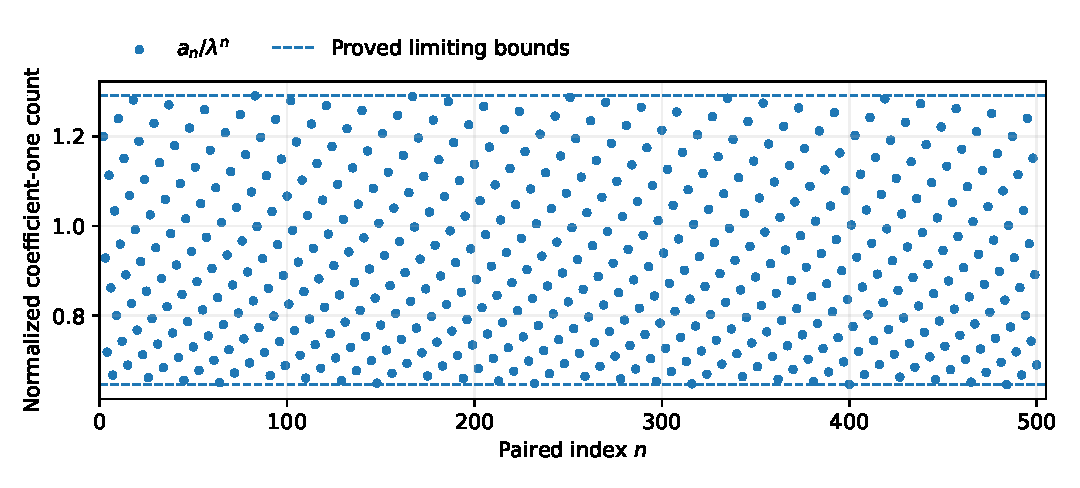
\includegraphics[width=0.97\linewidth]{figures/normalized_counts.pdf}
\caption{The normalized counts $a_n/\lambda^n$ for $2\le n\le500$.
The dashed lines are the limiting bounds in \eqref{eq:limitinterval}.
The nonvanishing oscillation is proved by irrational rotation, not inferred
from this plot. Floating-point arithmetic is used only to draw the figure.}
\label{fig:oscillation}
\end{figure}

\section{Dense singularities and a natural boundary}\label{sec:boundary}

The fluctuation law does more than prevent a constant leading asymptotic.
Every Fourier mode of the profile $h$ is nonzero. Each mode produces a
boundary singularity, and the corresponding points are dense on the circle
of convergence.

\subsection{A precise Abelian lemma}
\begin{lemma}[Ces\`aro means imply radial limits]\label{lem:abel}
Let $(c_n)$ be a bounded complex sequence. If
$M^{-1}\sum_{n=0}^{M-1}c_n\to c$, then
\begin{equation}\label{eq:abel}
 \lim_{\rho\uparrow1}(1-\rho)\sum_{n\ge0}c_n\rho^n=c.
\end{equation}
\end{lemma}
\begin{proof}
Put $S_N=\sum_{n=0}^Nc_n$. Absolute convergence for $0<\rho<1$ gives
\[
 \sum_{n\ge0}c_n\rho^n=(1-\rho)\sum_{N\ge0}S_N\rho^N.
\]
The hypothesis is $S_N=(N+1)c+o(N+1)$. Since
$\sum_{N\ge0}(N+1)\rho^N=(1-\rho)^{-2}$, the principal term contributes
$c$ after multiplying by $1-\rho$. For the error, fix $\varepsilon>0$ and
choose $N_0$ so that its absolute value is at most
$\varepsilon(N+1)$ for $N\ge N_0$. The tail contributes at most
$\varepsilon$, and the finitely many initial terms tend to zero. This
proves \eqref{eq:abel}.
\end{proof}

\subsection{Nonzero radial amplitudes at a dense set}
\begin{theorem}[Explicit dense boundary singularities]\label{thm:boundary}
For each $k\in\Z$, put $\omega_k=e^{-2\pi i k\alpha}$. Then
\begin{equation}\label{eq:radial}
 \lim_{\rho\uparrow1}(1-\rho)A(R\rho\omega_k)
 =\frac{2^{-\alpha}e^{2\pi i k\alpha}}{\log 2-2\pi i k}\ne0.
\end{equation}
The circle $|z|=R$ is a natural boundary of $A$.
\end{theorem}
\begin{proof}
Equation~\eqref{eq:growthroot} shows that the radius of convergence is
exactly $R$. Ignore the single correction at $n=1$ for the moment.
At $z=R\rho\omega_k$, formula \eqref{eq:profile} makes the summand
$h(u_n)\omega_k^n\rho^n$. Since
\[
 \omega_k^n=e^{2\pi i k\alpha}e^{-2\pi i k u_n},
\]
Lemma~\ref{lem:rotation}, applied to the Riemann integrable function
$h(u)e^{-2\pi i k u}$, gives the Ces\`aro mean
\begin{align*}
 \lim_{M\to\infty}\frac1M\sum_{n=0}^{M-1}h(u_n)\omega_k^n
 &=e^{2\pi i k\alpha}\int_0^1 2^{u-\alpha}e^{-2\pi i k u}\,du\\
 &=\frac{2^{-\alpha}e^{2\pi i k\alpha}}{\log2-2\pi i k}.
\end{align*}
In the integral, $e^{\log2-2\pi i k}-1=1$. The resulting value is nonzero
for every integer $k$. Lemma~\ref{lem:abel} proves \eqref{eq:radial}.
The omitted correction contributes $(1-\rho)R\rho\omega_k$, which tends
to zero.

If $A$ admitted a holomorphic extension across the point $R\omega_k$, it
would remain bounded along the inward radial segment near that point.
Equation~\eqref{eq:radial} contradicts this. Thus every $R\omega_k$ is a
singular point. Irrationality of $\alpha$ makes the set of $\omega_k$ dense
on the unit circle. An extension across any other point of $|z|=R$ would
be defined in an open neighborhood containing some $R\omega_k$, again a
contradiction. Hence no point on the circle admits analytic continuation
through the circle.
\end{proof}

The limit \eqref{eq:radial} describes a radial blowup. It does \emph{not}
assert that these are isolated poles or provide residues of a meromorphic
continuation: the singularities are dense, and no such neighborhood of
continuation is available.

\subsection{The full generating function and recurrence consequences}
\begin{corollary}\label{cor:fullboundary}
The circle $|t|=\sqrt R$ is a natural boundary of $F$.
\end{corollary}
\begin{proof}
Equation~\eqref{eq:fullrelation} makes $F$ holomorphic for
$|t|<\sqrt R$, with a removable singularity at zero. Suppose it extended
through some point $t_0$ on the boundary. Since $t_0\ne0$, the map
$t\mapsto t^2$ has a local analytic inverse near $t_0$. Also
$2t_0+1\ne0$: the only zero is $-1/2$, whereas
$\sqrt R>1/\sqrt2>1/2$. Solving \eqref{eq:fullrelation} for $A(t^2)$ would
therefore provide an analytic extension of $A$ through $t_0^2$, contrary
to Theorem~\ref{thm:boundary}.
\end{proof}

A power series $H(z)$ is D-finite if it satisfies a nonzero homogeneous
linear differential equation
\begin{equation}\label{eq:dfinite}
 p_d(z)H^{(d)}(z)+\cdots+p_0(z)H(z)=0,
 \qquad p_j(z)\in\C[z],\quad p_d\ne0.
\end{equation}
This is the standard terminology developed in \cite{StanleyDFinite}.
Away from the finitely many zeros of $p_d$, a linear differential equation
has analytic coefficients after division by $p_d$; its local solutions
continue along paths avoiding those zeros. An analytic germ satisfying
\eqref{eq:dfinite} cannot therefore have a natural boundary on a finite
circle.

Likewise, an algebraic germ has only finitely many possible finite
singularities. For an irreducible polynomial equation $p(z,H)=0$ of positive degree in $H$, exclude
the zeros of its leading coefficient in $H$ and of its discriminant in
$H$; the implicit-function theorem gives local analytic branches at the
remaining points. This also contradicts a natural boundary.

Finally, a sequence $(u_n)$ is P-recursive if it satisfies an eventual
nonzero linear recurrence with polynomial coefficients in $n$. Such a
recurrence implies a D-finite generating function. To recall the direct
mechanism, let $\theta=z\,d/dz$. Then $\theta(z^n)=nz^n$, so sums of
$p_j(n)u_{n+j}z^n$ can be written as differential operators in $\theta$
applied to $H(z)=\sum u_nz^n$, up to finitely many initial terms.
After clearing powers of $z$, the recurrence becomes a nonzero linear
differential equation with a polynomial right-hand side. Differentiating
sufficiently many times makes that right-hand side zero. These observations
and the two natural-boundary results prove all remaining conclusions of
Theorem~\ref{thm:main}.

\section{A complete classification for two bases}\label{sec:general}

The counterexample is part of a family in which the rationality question
can be answered exactly. Fix integers $2\le a<q$ and define the digit
polynomial
\begin{equation}\label{eq:digitpoly}
 D_a(y)=1+y+\cdots+y^{a-1}.
\end{equation}
Use the interleaved exponents
\begin{equation}\label{eq:generalexponents}
 G_{2j+1}=a^j,\qquad G_{2j+2}=q^j,
\end{equation}
and the products $\prod_{i=1}^N D_a(x^{G_i})$. This is precisely
\eqref{eq:stanleyproduct} with fixed $r=a-1$. The exponent generating
function is $t/(1-at^2)+t^2/(1-qt^2)$, and $G_N\to\infty$.
Let $v_{a,q}(N)$ count the coefficients equal to one and put
\[
 F_{a,q}(t)=\sum_{N\ge0}v_{a,q}(N)t^N.
\]
Two integers $a,q>1$ are \emph{multiplicatively dependent} when
$q^u=a^v$ for some positive integers $u,v$; equivalently,
$\log_q a$ is rational.

\begin{theorem}[Two-base rationality classification]\label{thm:classification}
For every pair of integers $2\le a<q$,
\begin{equation}\label{eq:classification}
 F_{a,q}(t)\text{ is rational}
 \quad\Longleftrightarrow\quad
 a\text{ and }q\text{ are multiplicatively dependent}.
\end{equation}
When $q^u=a^v$ with $u,v\ge1$, necessarily $v>u$, and
\begin{equation}\label{eq:eventualdependent}
 v_{a,q}(N+2v)=a^{v-u}v_{a,q}(N)
\end{equation}
for every sufficiently large $N$. In particular the reduced denominator
of $F_{a,q}(t)$ divides $1-a^{v-u}t^{2v}$.
\end{theorem}

\subsection{Exact counts for a general rectangle}
Write
\begin{equation}\label{eq:generalrectangle}
 Q^{a,q}_{m,n}(x)=
 \prod_{j=0}^{m-1}D_a(x^{a^j})
 \prod_{j=0}^{n-1}D_a(x^{q^j}),
\end{equation}
and let $U_{a,q}(m,n)$ be its number of coefficients equal to one.
The first product is $1+x+\cdots+x^{a^m-1}$. The second is supported,
with coefficient one, on the $a^n$ integers whose $n$ base-$q$ digits
belong to $\{0,\ldots,a-1\}$.

The sorted support is traversed by a base-$a$ counter interpreted in base
$q$. A carry through $t$ trailing maximal digits produces the gap
\begin{equation}\label{eq:generalgap}
 g_t=q^t-(a-1)\sum_{j=0}^{t-1}q^j
     =\frac{(q-a)q^t+a-1}{q-1}.
\end{equation}
It occurs
\begin{equation}\label{eq:generalmultiplicity}
 (a-1)a^{n-1-t}
\end{equation}
times: there are $a-1$ choices for the incremented nonmaximal digit and
$a^{n-1-t}$ choices for the higher digits. Because $q>a$, the gap sizes
are strictly increasing, beginning with $g_0=1$. A nonunit gap is
preceded and followed by unit gaps, and the first and last gaps are
unit, just as in Lemma~\ref{lem:ternarygaps}.

Define the exact threshold
\begin{align}
 T_{a,q}(m)
 &=\min\{t\ge0:(q-a)q^t+a-1\ge(q-1)a^m\}\label{eq:generalthreshold}\\
 &=\ceil{\log_q\!\left(\frac{(q-1)a^m-(a-1)}{q-a}\right)}.
 \label{eq:generallogthreshold}
\end{align}
The ceiling expression is an identity over the real numbers; the integer
inequality in \eqref{eq:generalthreshold} is the appropriate computational
definition.

\begin{proposition}[General rectangular formula]\label{prop:generalcount}
For $m,n\ge1$,
\begin{equation}\label{eq:generalcount}
 U_{a,q}(m,n)=2a^{\max(0,n-T_{a,q}(m))}.
\end{equation}
The empty-product cases are
$U_{a,q}(m,0)=a^m$ and $U_{a,q}(0,n)=a^n$.
\end{proposition}
\begin{proof}
Use Corollary~\ref{cor:isolated} with interval length $a^m$.
If $T=T_{a,q}(m)<n$, the number of gaps of size at least $a^m$ is
\[
 H=\sum_{t=T}^{n-1}(a-1)a^{n-1-t}=a^{n-T}-1.
\]
Otherwise $H=0$. In either case $2+2H$ is \eqref{eq:generalcount}.
The boundary cases follow from unique base expansions.
\end{proof}

For clarity, the factor $2$ in \eqref{eq:generalcount} is not replaced by
$a$: it counts the two uniquely covered endpoints associated with each
large gap, together with the two outer boundary contributions.

\subsection{Multiplicative independence forces nonrationality}
The gaps satisfy
\begin{equation}\label{eq:gaprec}
 g_{t+1}=qg_t-(a-1).
\end{equation}
For $m\ge1$, if $g_t\ge a^m$, then
\[
 g_{t+1}\ge qa^m-(a-1)\ge a^{m+1},
\]
because $(q-a)a^m\ge a-1$. Hence
\begin{equation}\label{eq:generalstep}
 T_{a,q}(m+1)-T_{a,q}(m)\in\{0,1\}\qquad(m\ge1).
\end{equation}
The restriction $m\ge1$ is necessary for this assertion: for example,
$T_{3,4}(0)=0$ and $T_{3,4}(1)=2$.
From \eqref{eq:generallogthreshold},
\begin{equation}\label{eq:generalslope}
 \frac{T_{a,q}(m)}{m}\longrightarrow\log_q a<1.
\end{equation}

For $n\ge1$, the even subsequence is
\[
 v_{a,q}(2n)=2a^{e_n},\qquad
 e_n=\max(0,n-T_{a,q}(n)).
\]
By \eqref{eq:generalstep}, the increments of $e_n$ belong to $\{0,1\}$;
by \eqref{eq:generalslope}, $e_n/n\to1-\log_q a$.
If $a,q$ are multiplicatively independent, this limit is irrational.
Apply Lemma~\ref{lem:finitefield} with $C=2$ and $b=a$ to conclude that
the even-section generating function is not rational. Then $F_{a,q}$ is
not rational either.

\subsection{Multiplicative dependence gives an eventual recurrence}
Suppose $q^u=a^v$ for positive integers $u,v$. Since $a<q$, necessarily
$u<v$. Put
\[
 M=a^v=q^u,\qquad K=\frac{q-1}{q-a},\qquad D=\frac{a-1}{q-a}.
\]
Writing $m=v\ell+r$ with $0\le r<v$, the inequality defining
$T_{a,q}(m)$ is
\begin{equation}\label{eq:depfirst}
 q^t\ge K a^{v\ell+r}-D.
\end{equation}
Set $t=u\ell+s$ and divide by $M^\ell$ to obtain
\begin{equation}\label{eq:depresidue}
 q^s\ge K a^r-DM^{-\ell}.
\end{equation}
For each residue $r$, let
\begin{equation}\label{eq:sr}
 s_r=\ceil{\log_q(K a^r)}.
\end{equation}
We have $q^{s_r-1}<K a^r\le q^{s_r}$. The positive distance between
$K a^r$ and $q^{s_r-1}$ is fixed, whereas $DM^{-\ell}\to0$.
Thus, for all sufficiently large $\ell$, the least integer $s$ satisfying
\eqref{eq:depresidue} is exactly $s_r$.
This remains true when $K a^r$ itself is an exact power of $q$; the
strict lower inequality is still available.
Therefore
\begin{equation}\label{eq:thresholdperiod}
 T_{a,q}(v\ell+r)=u\ell+s_r
 \quad\hbox{for all sufficiently large $\ell$},
\end{equation}
and, uniformly over the finitely many residues,
\begin{equation}\label{eq:Tshift}
 T_{a,q}(m+v)=T_{a,q}(m)+u
 \quad\hbox{for all sufficiently large $m$}.
\end{equation}

Because $\log_q a<1$, the maxima in \eqref{eq:generalcount} no longer
truncate for either $m=n$ or $m=n+1$ once $n$ is large enough.
Increasing the full product length by $2v$ increases both rectangular
indices by $v$; equation \eqref{eq:Tshift} then increases the exponent of
$a$ in \eqref{eq:generalcount} by $v-u$. This proves
\eqref{eq:eventualdependent} on both parities.
Multiplying the generating function by $1-a^{v-u}t^{2v}$ leaves only
finitely many nonzero coefficients, so it is a polynomial.
This proves the rational direction and completes
Theorem~\ref{thm:classification}.

\subsection{Rational controls and explicit examples}
The classification is not simply a separation between equal and unequal
bases. Different bases can be dependent: for example, $4^3=8^2$.
Table~\ref{tab:dependent} records several eventual recurrences used as
computational controls.

\begin{table}[htbp]
\centering
\caption{Dependent-base controls. Each displayed recurrence is eventually
valid; the verification suite checks every $40\le N\le200$.}
\label{tab:dependent}
\begin{tabular}{rrcl}
\toprule
$a$&$q$&Relation&Eventual recurrence\\
\midrule
2&4&$4=2^2$&$v_{2,4}(N+4)=2v_{2,4}(N)$\\
2&8&$8=2^3$&$v_{2,8}(N+6)=4v_{2,8}(N)$\\
3&9&$9=3^2$&$v_{3,9}(N+4)=3v_{3,9}(N)$\\
4&8&$8^2=4^3$&$v_{4,8}(N+6)=4v_{4,8}(N)$\\
4&16&$16=4^2$&$v_{4,16}(N+4)=4v_{4,16}(N)$\\
8&16&$16^3=8^4$&$v_{8,16}(N+8)=8v_{8,16}(N)$\\
9&27&$27^2=9^3$&$v_{9,27}(N+6)=9v_{9,27}(N)$\\
\bottomrule
\end{tabular}
\end{table}

For a particularly simple closed form, take $a=2$ and $q=2^s$ with
$s\ge2$. For $n\ge1$, writing $n=s\ell+r$, $0\le r<s$, one has
$g_\ell<2^n\le g_{\ell+1}$. Indeed,
$g_\ell<q^\ell\le2^n$ when $\ell\ge1$, while $g_0=1<2^n$ when
$\ell=0$; and
\[
 g_{\ell+1}=\frac{(q-2)q^{\ell+1}+1}{q-1}
 \ge\frac{q^{\ell+1}}2\ge2^n.
\]
It follows that $T_{2,2^s}(n)=\floor{n/s}+1$ and
\begin{equation}\label{eq:powertwoeven}
 v_{2,2^s}(2n)=2^{n-\lfloor n/s\rfloor}\qquad(n\ge0).
\end{equation}
Summing by residue classes gives
\begin{equation}\label{eq:powertworational}
 \sum_{n\ge0}v_{2,2^s}(2n)z^n
 =\frac{\sum_{j=0}^{s-1}2^jz^j}{1-2^{s-1}z^s}.
\end{equation}
In contrast, every pair $(2,q)$ with $q>2$ not a power of $2$ gives a
counterexample with the original binary factors $1+x^{G_i}$.

\section{Reproducible exact computations}\label{sec:computations}

The proof does not infer an infinite statement from a long prefix. The
computations serve three narrower purposes: validating the indexing and
exceptional cases, checking the finite combinatorial identities by
independent representations, and making the derived integer sequences easy
to reuse.

\subsection{Three distinct computational representations}
The module \texttt{code/mixed\_base.py} implements three routes.
Direct multiplication stores every coefficient and multiplies by the digit
factors from their definition. An endpoint sweep independently enumerates
the sparse digit support and adds $+1$ at each interval start and $-1$ at
each interval end; it computes the histogram of \emph{all} coefficient
values. The closed formula computes only the threshold and the resulting
power of $a$. The first method does not use the interval model, and the
second does not use the carry-gap counting formula.

The checker compares entire histograms when feasible, not merely their
coefficient-one totals. It also checks total degree and the mass identity
\[
 \sum_s[x^s]Q^{a,q}_{m,n}(x)=Q^{a,q}_{m,n}(1)=a^{m+n}.
\]
The zero-coefficient histogram entry refers only to exponents between zero
and the polynomial's degree; infinitely many trailing zero coefficients
are never counted.

\begin{table}[htbp]
\centering
\caption{Executed finite verification. All decisions use exact integers.}
\label{tab:verification}
\begin{tabular}{>{\raggedright\arraybackslash}p{0.65\linewidth}r}
\toprule
Check&Instances\\
\midrule
Dense rectangle: direct histogram = sweep histogram; count = formula&625\\
Larger binary--ternary rectangle: sweep count and mass identities&384\\
Enumerated carry-gap multiplicities and adjacency&150\\
Actual interleaved prefixes $P_0,\ldots,P_{24}$&25\\
Threshold compared with both adjacent integer powers&149\,050\\
Exact floor-formula identities, $0\le n\le10\,000$&10\,001\\
Input recurrence \eqref{eq:inputrec}&1\,000\\
Even--odd identity \eqref{eq:odd}&1\,000\\
Dependent-family recurrence, seven families and $161$ indices each&1\,127\\
\bottomrule
\end{tabular}
\end{table}

The dense grid uses $2\le a\le6$, $a+1\le q\le a+5$, and
$0\le m,n\le4$. The larger sweep grid uses $(a,q)=(2,3)$,
$1\le m\le24$, and $1\le n\le16$. The carry checks enumerate
$1\le n\le6$ for the same $25$ base pairs as the dense grid.
The threshold tests cover $0\le m\le100\,000$ for $(2,3)$ and
$0\le m\le1000$ for $49$ additional enumerated base-pair cases
($2\le a\le8$ and $a+1\le q\le a+7$; this includes $(2,3)$ again).
The largest directly expanded polynomial has degree $269\,815$.

The supplied run completed successfully. The file
\texttt{data/verification.json} records the counts, the actual elapsed time,
and a SHA-256 digest of the dense-grid histograms. Timing is an observation
about the supplied execution environment, not a performance guarantee.

\subsection{Exact thresholds, not floating-point logarithms}
The following compact function computes any full-prefix count in the
family. It is an executable form of Proposition~\ref{prop:generalcount}.
\begin{lstlisting}
def count_one_prefix(N: int, a: int = 2, q: int = 3) -> int:
    if N < 0 or not 2 <= a < q:
        raise ValueError("Need N >= 0 and integer bases 2 <= a < q")
    m, n = (N + 1) // 2, N // 2
    if n == 0:
        return a**m
    if m == 0:
        return a**n
    t, q_power = 0, 1
    target = (q - 1) * a**m
    while (q - a) * q_power + a - 1 < target:
        q_power *= q
        t += 1
    return 2 * a**max(0, n - t)
\end{lstlisting}
The full module also offers a streaming threshold computation that reuses
$a^m$ and $q^{T(m)}$. For fixed bases, the first $M$ thresholds need
$O(M)$ comparisons and multiplications by fixed integers, with $O(M)$-bit
working integers. In a bit-cost model with linear-cost fixed-integer
multiplication, this gives an $O(M^2)$ upper bound on total bit operations
and $O(M)$ working bits when results are streamed. Materializing all large
output integers may itself require quadratic total space in bits.

For a single rectangle, direct dense expansion has a degree that grows
exponentially in the sparse-digit length. The sweep instead uses
$O(a^n)$ endpoint events and the implementation sorts them in
$O(a^n\log(a^n))$ comparisons. The formula avoids both enumerations.
These counts describe arithmetic or comparison operations; they do not
treat arbitrarily large integer operations as constant-time in the
bit-complexity discussion.

\subsection{Package contents and reproduction}
Run the verification suite from the project directory with
\begin{lstlisting}
python code/verify.py
\end{lstlisting}
It requires only the Python standard library and is written for Python
3.9 or later. Do not run it with \texttt{-O}, which disables assertions.
The supplied verification was executed using Python 3.13.
The command
\begin{lstlisting}
python code/mixed_base.py 40 --a 2 --q 3
\end{lstlisting}
prints the first $41$ full-prefix counts.
The CSV files contain indices $0$ through $1000$; a separate plain-text
file uses the familiar two-column sequence format. No OEIS identifier is
assigned or claimed.

The PDF is built with two passes of \texttt{pdflatex article.tex}; all
needed figure PDFs are included. Recreating the figures with
\texttt{python code/make\_figures.py} additionally requires Matplotlib.
The plots use floating-point arithmetic only for visualization; all
verification decisions and all exported integer sequence values are exact.
The README gives the complete directory map and reproduction commands.

\section{What is settled, and what remains}\label{sec:scope}

The universal implication in \eqref{eq:hypotheses}--\eqref{eq:stanleyproduct}
is false. The counterexample uses positive integer exponents tending to
infinity, a fourth-order constant-coefficient recurrence for those exponents,
fixed binary factors, and the simplest nonzero coefficient value $k=1$.
The output generating function not only fails to be rational: it has a
natural boundary and is not D-finite. Within the specified two-base digit
family, Theorem~\ref{thm:classification} gives a complete rationality
classification.

Three boundaries of this result should be kept separate. First, the
exponents in the counterexample are not eventually increasing. The same
is true of the general interleaving when $a<q$: eventually $q^j>a^{j+1}$,
so each sufficiently late even-to-odd step decreases. Reordering all
exponents would preserve a finite product with a fixed multiset of
factors, but it changes the prefix sequence and need not preserve the
rationality of the exponent generating function. Thus this construction
does not settle a separately imposed monotone version.

Second, the proofs count coefficients equal to one. They do not establish
a corresponding classification for every fixed $k>1$. For those values,
multiple neighboring intervals and their overlaps matter; the isolated-gap
identity alone no longer determines the answer.

Third, the classification concerns the family
$G_{2j+1}=a^j$, $G_{2j+2}=q^j$ with digit set $0,\ldots,a-1$.
It is not a classification of all C-finite exponent sequences.
The arithmetic mechanism suggests studying which recurrence families
force periodic relative scales and which allow irrational threshold
frequencies, but no claim about all such families is made here.

These are directions left untouched by this report, not assertions that
each associated broader question has independently been verified to be
open in the literature. The completed result is the explicit counterexample,
its natural-boundary strengthening, and the exact two-base classification.

\begin{thebibliography}{9}
\raggedright

\bibitem{StanleyMO}
Richard Stanley,
\emph{A conjectured rational generating function},
MathOverflow question 431075, September 23, 2022.
\url{https://mathoverflow.net/questions/431075/a-conjectured-rational-generating-function}.
Source page inspected September 19, 2026.

\bibitem{StanleyRational}
Richard P. Stanley,
\emph{Theorems and Conjectures on Some Rational Generating Functions},
arXiv:2101.02131, version 3, September 30, 2021, 25 pp.
\url{https://arxiv.org/abs/2101.02131}.

\bibitem{StanleyDFinite}
Richard P. Stanley,
\emph{Differentiably Finite Power Series},
European Journal of Combinatorics \textbf{1} (1980), 175--188.
Author-hosted copy:
\url{https://math.mit.edu/~rstan/pubs/pubfiles/45.pdf}.

\end{thebibliography}
\end{document}
